% !TeX root = RJwrapper.tex
\title{munsell: Munsell colours in R}
\author{by Charlotte Wickham}

\maketitle

\abstract{
An abstract of less than 150 words.
}

\subsection{The munsell Packgage}\label{the-munsell-packgage}

\textbackslash{}begin\{Schunk\} \textbackslash{}begin\{Sinput\}
knitr::opts\_chunk\$set(echo = FALSE, message = FALSE, results =
``hide'') library(munsell) \textbackslash{}end\{Sinput\}
\textbackslash{}end\{Schunk\}

\section{Introduction}\label{introduction}

The \CRANpkg{munsell} package provides easy access to, and manipulation
of, the Munsell colours. The \pkg{munsell} package provides a mapping
between Munsell's orginal notation (e.g. ``5R 5/10'') and hexidecimal
strings suitable for use directly in R graphics. The package also
provides utilities to explore slices through the Munsell colour tree, to
transform Munsell colours and display colour palettes.

Munsell devised his system of colour notation to match the three
percetual dimensions of colour: hue, value and chroma. His notation
provides a naming scheme to colours that eases the choice of color
according to a specific purpose. His century old advice is still
relevent for the producers of statistical graphics and the munsell
package aims to enable user to easily follow it.

This vignette starts with an overview of the Munsell colour system,
followed by basic use of the munsell package. It follows with a survey
of advice for using colour and finshes with the technicalities of
converting Munsell colours to sRGB.

\subsection{Other colour packages}\label{other-colour-packages}

This vignette is designed for people interested in learning more about
the Munsell colour system and who are interested in putting together
their own palettes of colours. If you are looking for a prespecified
discrete set of colours you might be interested in the following R
packages:

\begin{itemize}
\item
  \CRANpkg{ggthemes} \citep{Arnold:2014aa} contains colour schemes that
  match the themes of publications or software, including some with
  perceptual backing (e.g. \texttt{theme\_few} based on Stephen Few's
  guideline for practical rules of colour) and others that aren't (e.g.
  \texttt{theme\_excel} if you are craving that Excel feeling)
\item
  \CRANpkg{wesanderson} \citep{Ram:2014aa} provides palettes of colours
  that typify various Wes Anderson films.
\item
  \pkg{RSkittleBrewer} \citep{Frazee:2014aa} provides palettes that
  match skittle varieties; when you need your plots induce salivation.
\item
  \CRANpkg{RColorBrewer} \citep{Neuwirth:2011aa} an R implementation of
  Cynthia Brewer's palette for maps
\end{itemize}

Another alternative approach to generating qualitative, sequential and
diverging colour palettes using the HCL colour space is described in
\citet{Zeileis:2009aa} and implemented in the \CRANpkg{colorspace}
package \citep{Ross-Ihaka:2013aa}. A brief comparison between the
Munsell colour space and the HCL colourspace is given in Section ?.

\subsection{The Munsell colour system}\label{the-munsell-colour-system}

Munsell developed a system that not only could precisely specify a
colour, but also provide a cognitive tool to help develop an
appreciation for a balance of colour. His system revolved around the
three perceptual dimensions of: hue, value and chroma. He imagined the
space spanned by these three dimensions being described by a sphere. At
the north pole lay white and at the south black, the greys lying on the
vertical axis between them. Position on this vertical axis describes a
color's \dfn{value}. \dfn{Hues} lie in a circle around this axis in the
wavelength order: red, yellow, green, blue, purple. The distance from
the axis is termed \dfn{chroma} and quantifies the intensity of the
colour. An image from ``A Grammar of Color'' \citep{Munsell:1921aa}
illustrating the axis of grey and arrangment of hue and chroma is
reproduced below. Consequently, any colour can be placed in the sphere
given its hue, value and chroma coordinates.

\includegraphics{munsell-axis.pdf}

The coordinate of value is a number between 0 (black) and 10 (white),
the coordinate of chroma was also orignally a number between 0 (grey)
and 10 (pigment of maximal strength), but as new stronger pigments were
discovered, the scale has expanded beyond 10 (up to 24 in
\pkg{munsell}). Hues are specified by one of ten character hue codes (R,
YR, Y, GY, G, BG, B, PB, P, RP) matching Munsell's five principal hues
(Red, Yellow, Green, Blue and Purple) and their intermediates
(Yellow-Red, Green-Yellow, Blue-Green, Purple-Blue and Red-Purple) and a
number between 0 and 10, that further divides the distance between a
principal hue and it's neighbouring intermediate into 10 steps, where 5
denotes a colour typical of the hue. In addition greys (any colour with
0 chroma) are specified by the hue code N (without a number). A colour
is then specified by a string of the form ``H V/C'', for example ``5R
5/10'' which specifies a red equidistant between yellow-red and
red-purple of middle value and chroma 10.

Munsell recognised that the true space of colours was anything but
spherical. Hues vary widely in their chroma, there exist reds of middle
value that extend much farther from the central axis of the sphere, than
do their opposite Blue-Greens. He likened the true colour space to that
of a tree, with some branches extending from the central trunk of grey's
much farther at certain combinations of hue and value than others. He
illustrated this in his Colour Atlas, first published in XXXX, that
consisted of a set of physical paint swatches that explored horizontal
and vertical slices through his colour space. For example, his chart for
``5R'', a red, from the atlas is reproduced below along with the
replication of the chart using the munsell function
\texttt{complement\_slice("5R")}.

\begin{figure}
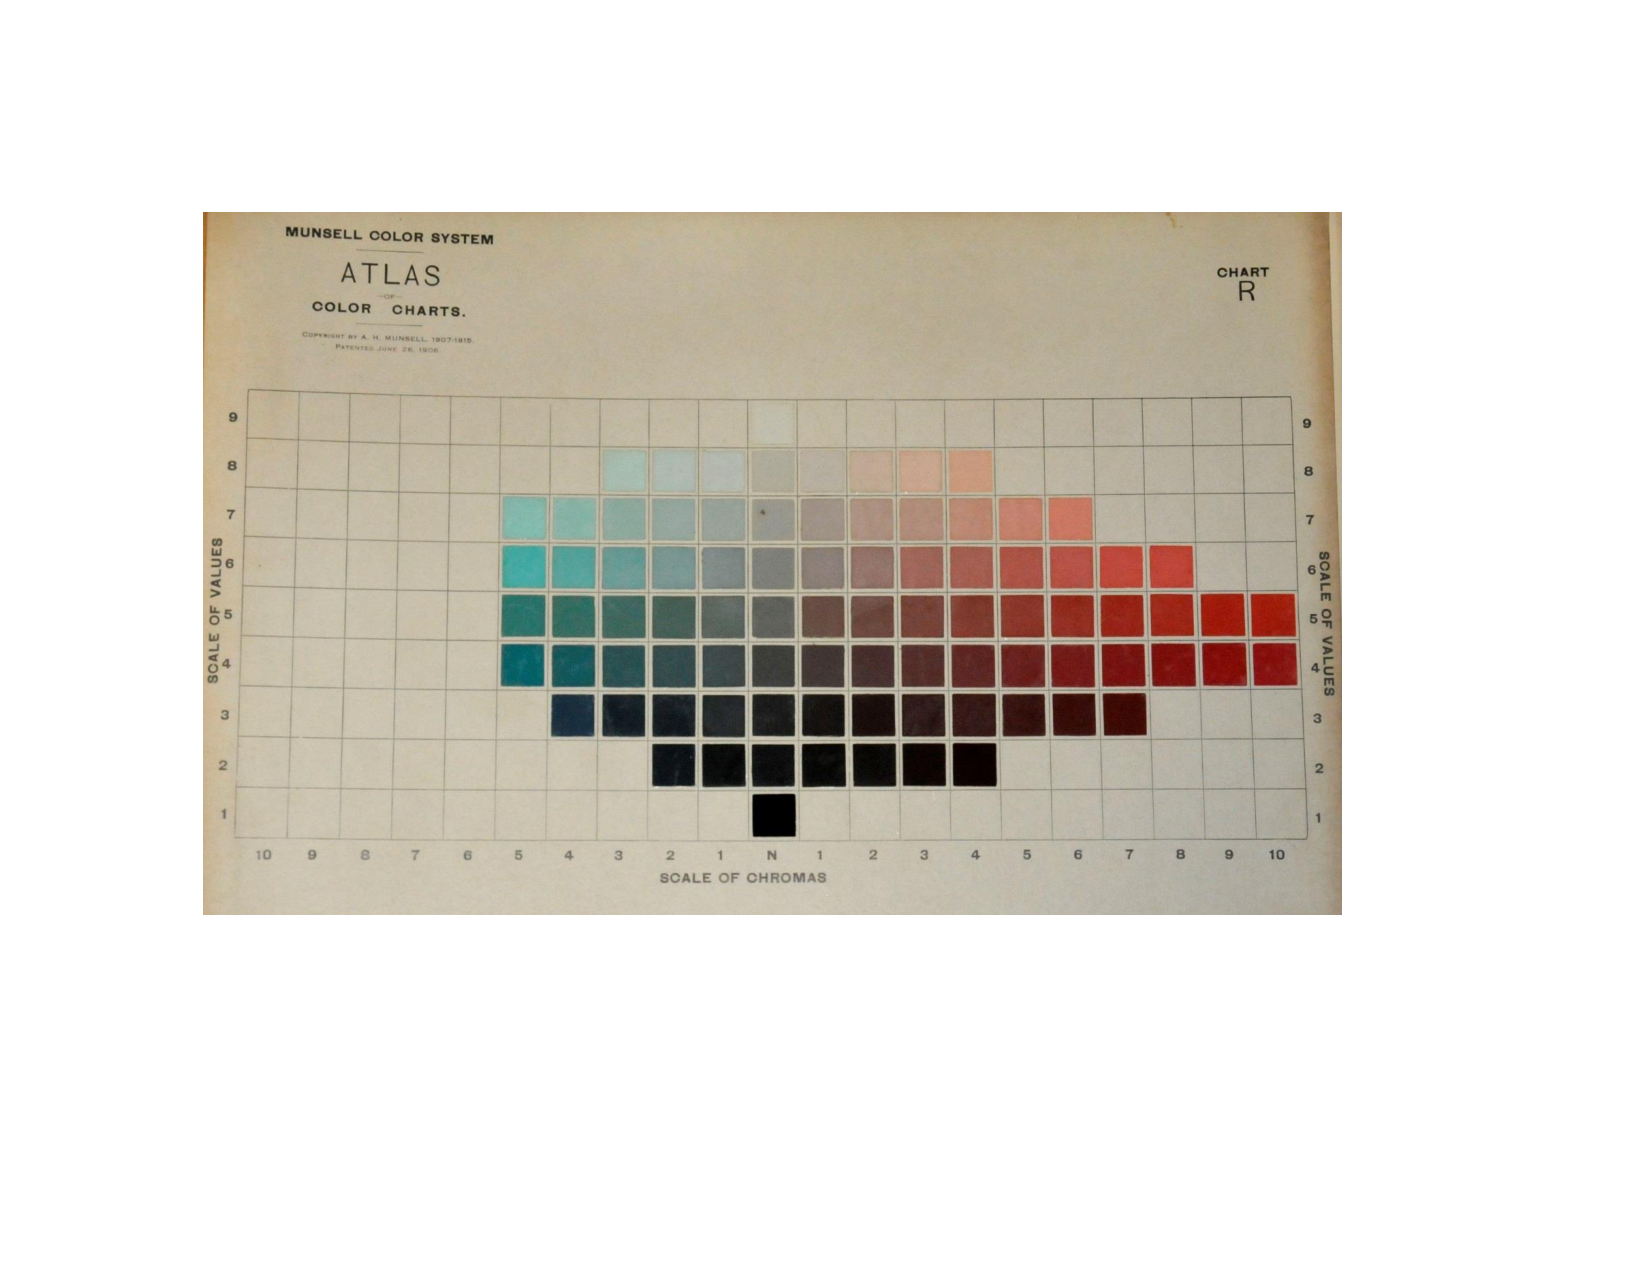
\includegraphics[width=0.45\textwidth]{munsell-atlas-chart-r}
\begin{Schunk}

\includegraphics[width=0.45\textwidth]{intro_files/figure-latex/unnamed-chunk-2-1} \end{Schunk}
\end{figure}

\section{The munsell package}\label{the-munsell-package}

Functions in \CRANpkg{munsell} fall into three basic use categories:
specifying Munsell colours, altering Munsell colours and exploring the
Munsell color space.

\subsection{Color specification}\label{color-specification}

Following Munsell, specifying colours is done with a specific string
format: ``H V/C'' where H is a hue code (see \code{mnsl\_hues()} for a
list of those available, excluding ``N''), V an integer in \([0, 10]\)
specifying value, and C an even integer specifying chroma. The
\code{mnsl} function takes the string and returns a hexadecimal RGB
representation:

\begin{Schunk}
\begin{Sinput}
mnsl("5R 5/10")
\end{Sinput}
\begin{Soutput}
#> [1] "#C65858"
\end{Soutput}
\end{Schunk}

Visually examining a colour can either be done by using \code{mnsl} with
a base plotting call, or using \texttt{plot\_mnsl} which plots colour
swatches using \CRANpkg{ggplot2}:

\begin{Schunk}
\begin{Sinput}
plot.new()
rect(0, 0, 1 ,1 , col = mnsl("5R 5/10"))
plot_mnsl("5R 5/10")
\end{Sinput}
\end{Schunk}

\emph{Where to look for using colours in ggplot2, lattice, base and
ggvis}

\subsection{Colour manipulation}\label{colour-manipulation}

\CRANpkg{munsell} provides convenience functions that alter a colour by
taking steps in the hue, value and chroma dimensions: \code{rygbp},
\code{pbgyr},\code{lighter}, \code{darker}, \code{saturate} and
\code{desaturate}.\\

\begin{Schunk}

\includegraphics{intro_files/figure-latex/unnamed-chunk-5-1} \end{Schunk}

Each function optionally takes the number of steps to take in the
dimension and consequently are easily used to create scales in a
particular dimension.\\

\begin{Schunk}
\begin{Sinput}
p <- plot_mnsl(sapply(0:6, darker, col = "5PB 7/4"))
p + facet_wrap(~ num, nrow = 1)
\end{Sinput}

\includegraphics{intro_files/figure-latex/unnamed-chunk-6-1} \end{Schunk}

\subsection{Colour space exploration}\label{colour-space-exploration}

Slices through the colour space of constant hue, chroma or value can be
displayed using the functions: \code{hue\_slice}, \code{chroma\_slice}
and \code{value\_slice}. Additionally \code{complement\_slice} displays
a slice of constant hue, alongside a slice of it's complement, the hue
that is on the opposite side of the colour sphere to that specified.

\begin{tabular}{ll}
  \toprule
  \multicolumn{2}{l}{\textbf{Altering colours}} \\
     & \code{darker} \\
     & \code{lighter} \\
     & \code{saturate} \\
     & \code{desaturate} \\
     & \code{rygbp} \\
     & \code{pbgyr}\\
     & \code{complement}\\
  \multicolumn{2}{l}{\textbf{Converting colours}} \\   
    & \code{mnsl}/\code{mnsl2hex} \\
    & \code{hvc2mnsl} \\
    & \code{rgb2mnsl} \\
  \multicolumn{2}{l}{\textbf{Exploring the munsell color space}} \\       
    & \code{hue\_slice} \\
    & \code{value\_slice} \\
    & \code{chroma\_slice} \\
    & \code{complement\_slice} \\
  \multicolumn{2}{l}{\textbf{Utility functions}} \\     
    & \code{plot\_mnsl} \\
    & \code{plot\_closest} \\ 
\bottomrule
\end{tabular}

\section{\texorpdfstring{Building palettes using \pkg{munsell} and
Munsell's
advice}{Building palettes using  and Munsell's advice}}\label{building-palettes-using-and-munsells-advice}

This section explores a couple of examples of building a palette for a
specific purpose: choosing a discrete colour scale for a bar chart,
choosing a seqential scale for a heatmap, and choosing a diverging scale
for a chloropleth map.

\subsection{A discrete scale}\label{a-discrete-scale}

Consider the following bar chart using the Auckland University
Undergraduate Counts Data, \code{auuc}, from \CRANpkg{VGAM} created
using \CRANpkg{ggplot2}. In this situation where colour is encoding
categories, advice is generally to chose colours that have equal visual
weight (refs), interpreted to be of different hue, but constant chroma
and value. This is the default discrete colour mapping in
\CRANpkg{ggplot2}: equally spaced steps in hue with constant chroma and
luminance in the hcl colour space, and is displayed in panel in Figure
\ref{fig:qual}.

Let's choose another palette following this advice using the Munsell
colour space. Our first step is to choose appropriate levels for chroma
and value. Since value is perhaps the most readily imagined without
displaying colours, one might proceed by looking at slices through the
colour space for a given value, chosen based on whether a light or dark
palette is required. Let's start with a mid value palette:

\begin{Schunk}
\begin{Sinput}
value_slice(5) 
\end{Sinput}

\includegraphics{intro_files/figure-latex/unnamed-chunk-7-1} \end{Schunk}

It seems reasonable to choose hues that are easily dishtinguished, this
becomes a balance between the number of hues available at a given chroma
and the distinguisability of hues at a given chroma. For example, at
chroma level 2 (the central ring of colours in Figure \ref{fig:qual})
all hues are available, so four colours could be equally spaced through
the entire spectrum of colours, but hues with such low chroma are hard
to dishtinguish. In contrast, at chroma level 14, only hues from red
through purple blue are available (10R - 7.5PB), but even hues a couple
of steps apart are easy to distinguish at this level.

Palettes can be built on these extremes (and NOT reccomended):

\begin{Schunk}
\begin{Sinput}
pal_b <- mnsl(sapply(seq(0, 30, 10), rygbp, col = "5R 5/2"))
pal_c <- mnsl(sapply(seq(0, 9, 3), rygbp, col = "7.5PB 5/14"))
\end{Sinput}
\end{Schunk}

and are displayed in Figure \ref{fig:qual}. Both plots also incorporate
lines bounding each colour that contrast in value, ``N 4/0'' (Guideline
4.6 \citet{Ware:2013aa}). A couple of alternatives are also displayed.
In each case the process to obtain them was the same: a slice at
particular value was displayed (\code{chroma\_slice}), this display was
examined for a constant chroma ring that had a desirable range of hues,
the palette was generated by moving in a constant hue step from a
starting colour using \code{rygbp}.

\begin{Schunk}
\begin{Sinput}
pal_d <- mnsl(sapply(seq(0, 18, 6), rygbp, col = "10YR 8/8"))
pal_e <- mnsl(sapply(seq(0, 24, 8), rygbp, col = "7.5G 4/6"))
pal_f <- mnsl(sapply(seq(0, 12, 4), rygbp, col = "7.5R 6/6"))
\end{Sinput}
\end{Schunk}

\begin{Schunk}
\begin{figure}
\includegraphics[width=.49\linewidth]{intro_files/figure-latex/qual-1} \includegraphics[width=.49\linewidth]{intro_files/figure-latex/qual-2} \includegraphics[width=.49\linewidth]{intro_files/figure-latex/qual-3} \includegraphics[width=.49\linewidth]{intro_files/figure-latex/qual-4} \includegraphics[width=.49\linewidth]{intro_files/figure-latex/qual-5} \includegraphics[width=.49\linewidth]{intro_files/figure-latex/qual-6} \caption[Examples of quantitative palettes]{Examples of quantitative palettes: a) the \pkg{ggplot2} default, b)-f) generated using \pkg{munsell}}\label{fig:qual}
\end{figure}
\end{Schunk}

\subsection{Quantitative scales}\label{quantitative-scales}

\begin{Schunk}
\begin{Soutput}
#> Warning: Removed 29 rows containing missing values (geom_text).
\end{Soutput}

\includegraphics{intro_files/figure-latex/quant-1} \includegraphics{intro_files/figure-latex/quant-2} \includegraphics{intro_files/figure-latex/quant-3} \includegraphics{intro_files/figure-latex/quant-4} \includegraphics{intro_files/figure-latex/quant-5} \includegraphics{intro_files/figure-latex/quant-6} \end{Schunk}

A strategy for producing good quantitative palettes is to start with a
hue, then examine the slice of chroma and value at the hue for vertical,
horizontal or diagonal slices. As an example, three purple palettes are
shown in Figure \ref{fig:quant}. These generate sequential scales.
Diverging scales are simply produced by using two different hues joining
them with a common midpoint. A complememtary hue (the colour on the
opposite side of the hue circle) is a useful starting point. Two
palettes of this form are also shown in Figure \ref{fig:quant}.

Just discuss process: choose hue, examine \code{hue\_slice()} use
\code{darker}, \code{saturate}, or choose two hues.

spacing is not equal across dimensions, so a step in hue isn't
neccessarily as distinguishable as a step in value and/or chroma.

\section{Munsell colours in sRGB}\label{munsell-colours-in-srgb}

This section breifly discusses the translation between the Munsell
colour system, which first existed as physical paint swatches, and sRGB
the color system used for graphics devices in R. \pkg{munsell} relies
directly on the published tables in \citet{Newhall:1943aa} of CIE XYZ
(Illuminant C) values for Munsell colours. These tables were the result
of colour matching studies on Munsell's color samples along with some
smoothing and extrapolation with Munsell's goal of perceptually uniform
spacing in mind. The XYZ triplets in these tables are converted to R's
native sRGB triplets by first adapting the XYZ value to a different
white point (Illuminat C to D65) then using the \code{sRGB} function in
\CRANpkg{colorspace} to produce sRGB triplets.

The code that performs the conversion can be found in:

Currently the \texttt{munsell} package only includes hue in steps of
2.5, value in steps of 2 and chroma in steps of 1, corresponding
directly to the entries in Table 1 in \citet{Newhall:1943aa}. Other
values could be obtained by interpolation and this is an area for future
development.

Some physical paint swatches are not representable in sRGB; they lie
outside the colour range reproducible using the three primaries defined
by the sRGB space. These colours are not available in the munsell
package. \CRANpkg{munsell} generally allows operations on colours that
result in a non-representable color. This ensures operations that pass
through a non-representable color still work, e.g.
\code{lighter(saturate("2.5P 8/8"))}. Some limits apply,
\code{lighter(N 10/0)} will fail,
\code{saturate(destaurate("2.5P 8/2"))} will also fail. However, the
plotting functions will not display a non-representable colour, and a
warning is raised. The function \code{in\_gamut} can be used to identify
non-representable colours and the function \code{fix\_mnsl} to ``fix''
them by replacing them with a colour of the same hue and value but
chroma truncated to a representable level. For convenience, the plotting
functions include an argument, \code{fix} that will pass the colours
through \code{fix\_mnsl} before plotting them.

\section{A comparison with the hcl color
space}\label{a-comparison-with-the-hcl-color-space}

The hcl colorspace is polar transformation of the CIE 1976 (L\emph{, u},
v*) color space, an alternative to the Munsell system that also uses
three perceptual dimensions and attempts perceptually uniformity. For
comparison, Figure \ref{fig:hcl} displays a slice of the hcl colour
space when l = 80 (l, luminance ranges from 0 to 100 and plays the same
role as Munsell's lightness dimension). In addition points are added for
Munsell colours with a lightness of 8. These Munsell colours are plotted
at their h,c coordinates (obtained by moving from Munsell to sRGB to
hcl), Their luminance coordinates are not plotted, but deviated from 80
by less than 1.3. If the Munsell and hcl colorspaces were equivalent the
Munsell colours would appear evenly spaced on this plot. We see some
interesting features, the Munsell hues appear sparser in the
yellow-green and purple-red regions, the chroma spacing is much highest
in the oranges. What's the point?

In general using the hcl colorspace will result in smoother palettes,
but Munsell colours have perhaps a more intuitive colour naming scheme.

\begin{Schunk}

\includegraphics{intro_files/figure-latex/hcl-1} \end{Schunk}

\bibliography{munsell}

\address{
Charlotte Wickham\\
Oregon State University\\
Department of Statistics, 44 Kidder Hall\\ Corvallis, OR, USA 97330\\
}
\href{mailto:wickhamc@stat.oregonstate.edu}{\nolinkurl{wickhamc@stat.oregonstate.edu}}

